% 2018 江苏卷第22题：正三棱柱 ABC-A1B1C1
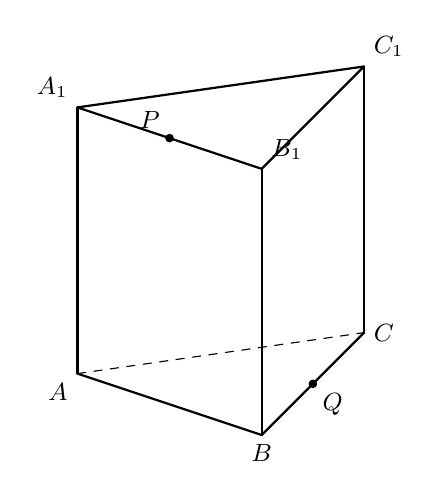
\begin{tikzpicture}[font=\small, line cap=round, line join=round, >=stealth, scale=1.3]
  % 底面顶点 A, B, C
  \coordinate (A) at (0, 0);
  \coordinate (B) at (1.8, -0.6);
  \coordinate (C) at (2.8, 0.4);

  % 顶面顶点
  \coordinate (A1) at (0, 2.6);
  \coordinate (B1) at (1.8, 2.0);
  \coordinate (C1) at (2.8, 3.0);

  % 中点 P (A1B1中点), Q (BC中点)
  \coordinate (P) at (0.9, 2.3);
  \coordinate (Q) at (2.3, -0.1);

  % 隐藏棱（虚线）
  \draw[dashed, thin] (A) -- (C);

  % 可见棱（实线）
  \draw[thick] (A) -- (B) -- (C);
  \draw[thick] (A1) -- (B1) -- (C1) -- cycle;
  \draw[thick] (A) -- (A1);
  \draw[thick] (B) -- (B1);
  \draw[thick] (C) -- (C1);

  % 标记点 P, Q
  \fill (P) circle (1.2pt) node[above left] {$P$};
  \fill (Q) circle (1.2pt) node[below right] {$Q$};

  % 顶点标签
  \node[below left] at (A) {$A$};
  \node[below] at (B) {$B$};
  \node[right] at (C) {$C$};
  \node[above left] at (A1) {$A_1$};
  \node[above right] at (B1) {$B_1$};
  \node[above right] at (C1) {$C_1$};
\end{tikzpicture}
